\documentclass[UTF8]{article}


\usepackage[zihao=-4]{ctex} % ctex可以写中文,中括号里那句的意思是正文小四号
\usepackage[a4paper]{geometry} % 调整纸张大小和页边距的包,这里中括号中规定了纸张大小
\usepackage{array}
\usepackage{fancyhdr}
\usepackage{amsmath}
\usepackage{multirow}
\geometry{left=2.5cm,right=2.5cm,top=2.5cm,bottom=2.5cm} % 页边距设置
\usepackage{caption}
\usepackage{wrapfig}
\usepackage{graphicx} % 用它在报告里加图
\graphicspath{{figures/}} % 指定图片所在文件夹
\pagestyle{fancy}
\rhead{测定空气比热容比}
\lhead{大学基础物理实验报告}
\cfoot{\thepage/4}
\rfoot{2023 年 3 月 10 日}

\begin{document}
	\thispagestyle{empty}
	\vspace*{0.5cm}
	
	\begin{figure}[h]
		\centering
		
\includegraphics[width=0.7\linewidth]{logo}
	\end{figure}
	\vspace*{0.1cm}
	\begin{center}
		\Huge{\textbf{大学基础物理实验报告}}\\
		\Huge{\textbf{《测定空气比热容比》}}
		
		\vspace*{0.1cm}
	\end{center}
	\begin{table}[h]
		\centering	
		\begin{Large}
			\begin{tabular}{p{3cm} p{5cm}<{\centering}}
				姓\qquad 名: & 蒋丰毅 \\
				\hline
				学\qquad 院: & 软件学院 \\
				\hline
				学\qquad 号: & 2211082 \\
				\hline
				分\qquad 组: & C组10号 \\
				\hline
				实验时间: & 2023.3.16\\
				\hline

			\end{tabular}
		\end{Large}
	\end{table}
	\clearpage
	\normalsize
	\begin{center}
		\LARGE\textbf{测定空气比热容比}
	\end{center}
	\subsection*{[实验目的要求]}
	\par 1.学习测定空气比定压热容与比定容热容之比的一种方法。
	\par 2.观察热学过程中状态变化及基本物理规律。
	\par 3.学习用传感器精确测定气体压强和温度的原理与方法。
	
	
	\subsection*{[实验仪器用具]}
	\par FD-NCD-Ⅱ空气比热容比测定仪,由机箱(含数字电压表二只)、储气瓶、传感器两只(电流型集成温度传感器AD590和扩散硅压力传感器各一只)等组成。
	\subsection*{[实验原理简述]}
	\par 物质的比热容分为压力恒定时的比定压比热容$c_p$,体积一定时的比定容比热容$c_V$,二者又称为主比热容,由于本实验实际过程中所设计的温度返回不大,二者近似为常量。固体,液体和气体的膨胀系数依次增大:对于气体而言,因膨胀而对外界做的功就不能忽略不计,故$c_p$与$c_V$必须严格区别。
	\par 理想气体存在方程:$c_p-c_V=R / M$,由此引出一个重要的物理量$\gamma$:
	\[\gamma=\frac{c_p}{c_V}=1+\frac{R}{M c_V} \]
	\par 其中$R$为气体普适常量,$M$表示气体的摩尔质量,$\gamma$称为气体的主比热容之比。
	
	\begin{wrapfigure}{r}{8cm}%靠文字内容的右侧
		\centering
		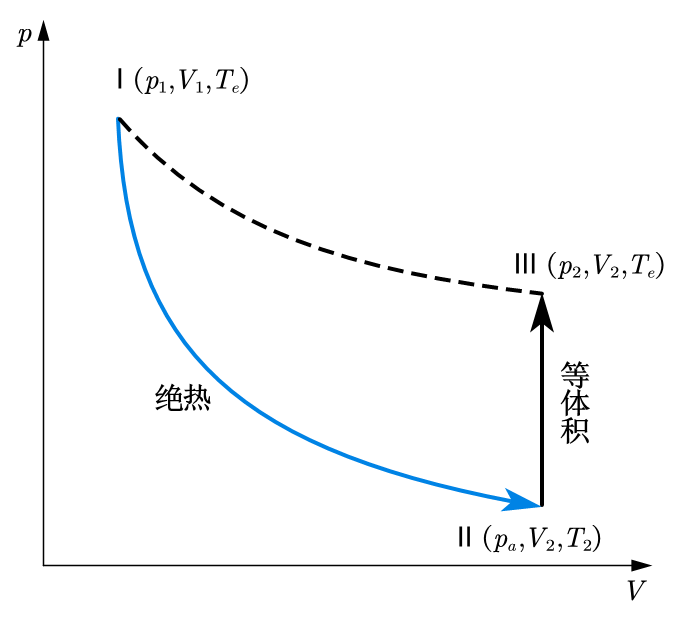
\includegraphics[width=0.5\textwidth]{p-V图}
		\caption{\footnotesize $p-V$图}
	\end{wrapfigure}
	\par 预测量$\gamma$值,需要三个状态。状态$\textup{\uppercase\expandafter{\romannumeral1}}$:以比大气压$p_a$稍高的压力$p_1$,向玻璃容器压入适量气体,并以与外部温度$T_e$相等之时单位质量的气体体积作为$V_1$。状态$\textup{\uppercase\expandafter{\romannumeral2}}$:急速打开放气活塞,使压强降至大气压$p_a$,由于是绝热膨胀,$T_2<T_e$.状态$\textup{\uppercase\expandafter{\romannumeral3}}$:关闭活塞后若再放置一段时间,系统将从外界吸收热量,且温度重新升高至$T_e$,由于体积不变,压力随之增加为$p_2$.
	\par 状态$\textup{\uppercase\expandafter{\romannumeral1}}\to\textup{\uppercase\expandafter{\romannumeral2}}$的变化是绝热的,故满足泊松公式
	\begin{equation*}
		p_1V_1^{\gamma}=p_2V_2^{\gamma}
	\end{equation*}
	\par 而状态$\textup{\uppercase\expandafter{\romannumeral3}}$与$\textup{\uppercase\expandafter{\romannumeral1}}$是等温的,故玻意耳定律成立
	\[ p_1V_1=p_2V_2\]
	\par 由前两个式子消去$V_1,V_2$,并求解得。
	\begin{equation}
		\gamma=\frac{\ln p_1-\ln p_{\mathrm{a}}}{\ln p_1-\ln p_2}=\frac{\ln \left(p_1 / p_{\mathrm{a}}\right)}{\ln \left(p_1 / p_2\right)}
	\end{equation}
	\par 若以$p_1^{\prime}$和$p_2^{\prime}$分别表示$p_1$与$p_a$及$p_2$与$p_a$的压力差,则有
	\begin{equation*}
	\left.\begin{array}{l}
		p_1=p_a+p_1^{\prime} \\
		p_2=p_a+p_2^{\prime}
	\end{array}\right\}
	\end{equation*}
	\par 将此式带入到(1)式,注意到$p_a\gg p_1^{\prime}>p_2^{\prime}$
	\begin{equation*}
		\ln p_1-\ln p_{\mathrm{a}}=\ln \frac{p_1}{p_{\mathrm{a}}}=\ln \left(1+\frac{p_1^{\prime}}{p_{\mathrm{a}}}\right) \approx \frac{p_1^{\prime}}{p_{\mathrm{a}}}
	\end{equation*}
	\par 以及
	\begin{equation*}
		\ln p_1-\ln p_2=\left(\ln p_1-\ln p_{\mathrm{a}}\right)-\left(\ln p_2-\ln p_{\mathrm{a}}\right)\approx \frac{p_1^{\prime}}{p_{\mathrm{a}}}-\frac{p_2^{\prime}}{p_{\mathrm{a}}}
	\end{equation*}
	\par 故
	\begin{equation}
		\gamma=\frac{p_1^{\prime}}{p_1^{\prime}-p_2^{\prime}}
	\end{equation}
	\par 故只需测得$p_1^{\prime}$以及$p_2^{\prime}$,即可通过(2)式求出空气的比热容比。
	\subsection*{[实验步骤]}
	\par 1.开启玻璃瓶的两个活塞并开启电子仪器的电源,使用调零旋钮将测定气压的表示数调整为$0mV$,预热20分钟。
	\par 2.关闭出气活塞,使用橡皮球往玻璃瓶中压入大约$120mV$气体后,关闭进气活塞,等待直到电压表示数稳定,记录此时电压表的示数为$p^{\prime}_1$,温度表的示数为$T_1$。
	\par 3.打开出气活塞,待放气声音停止后立即关闭,等待直到电压表的示数稳定,记录电压表示数为$p^{\prime}_2$,温度表示数为$T_2$。
	\par 4.重新打开两个活塞,重复步骤1和2.
	\subsection*{[数据处理]}
	\par
		\begin{figure}[h]
		\centering
		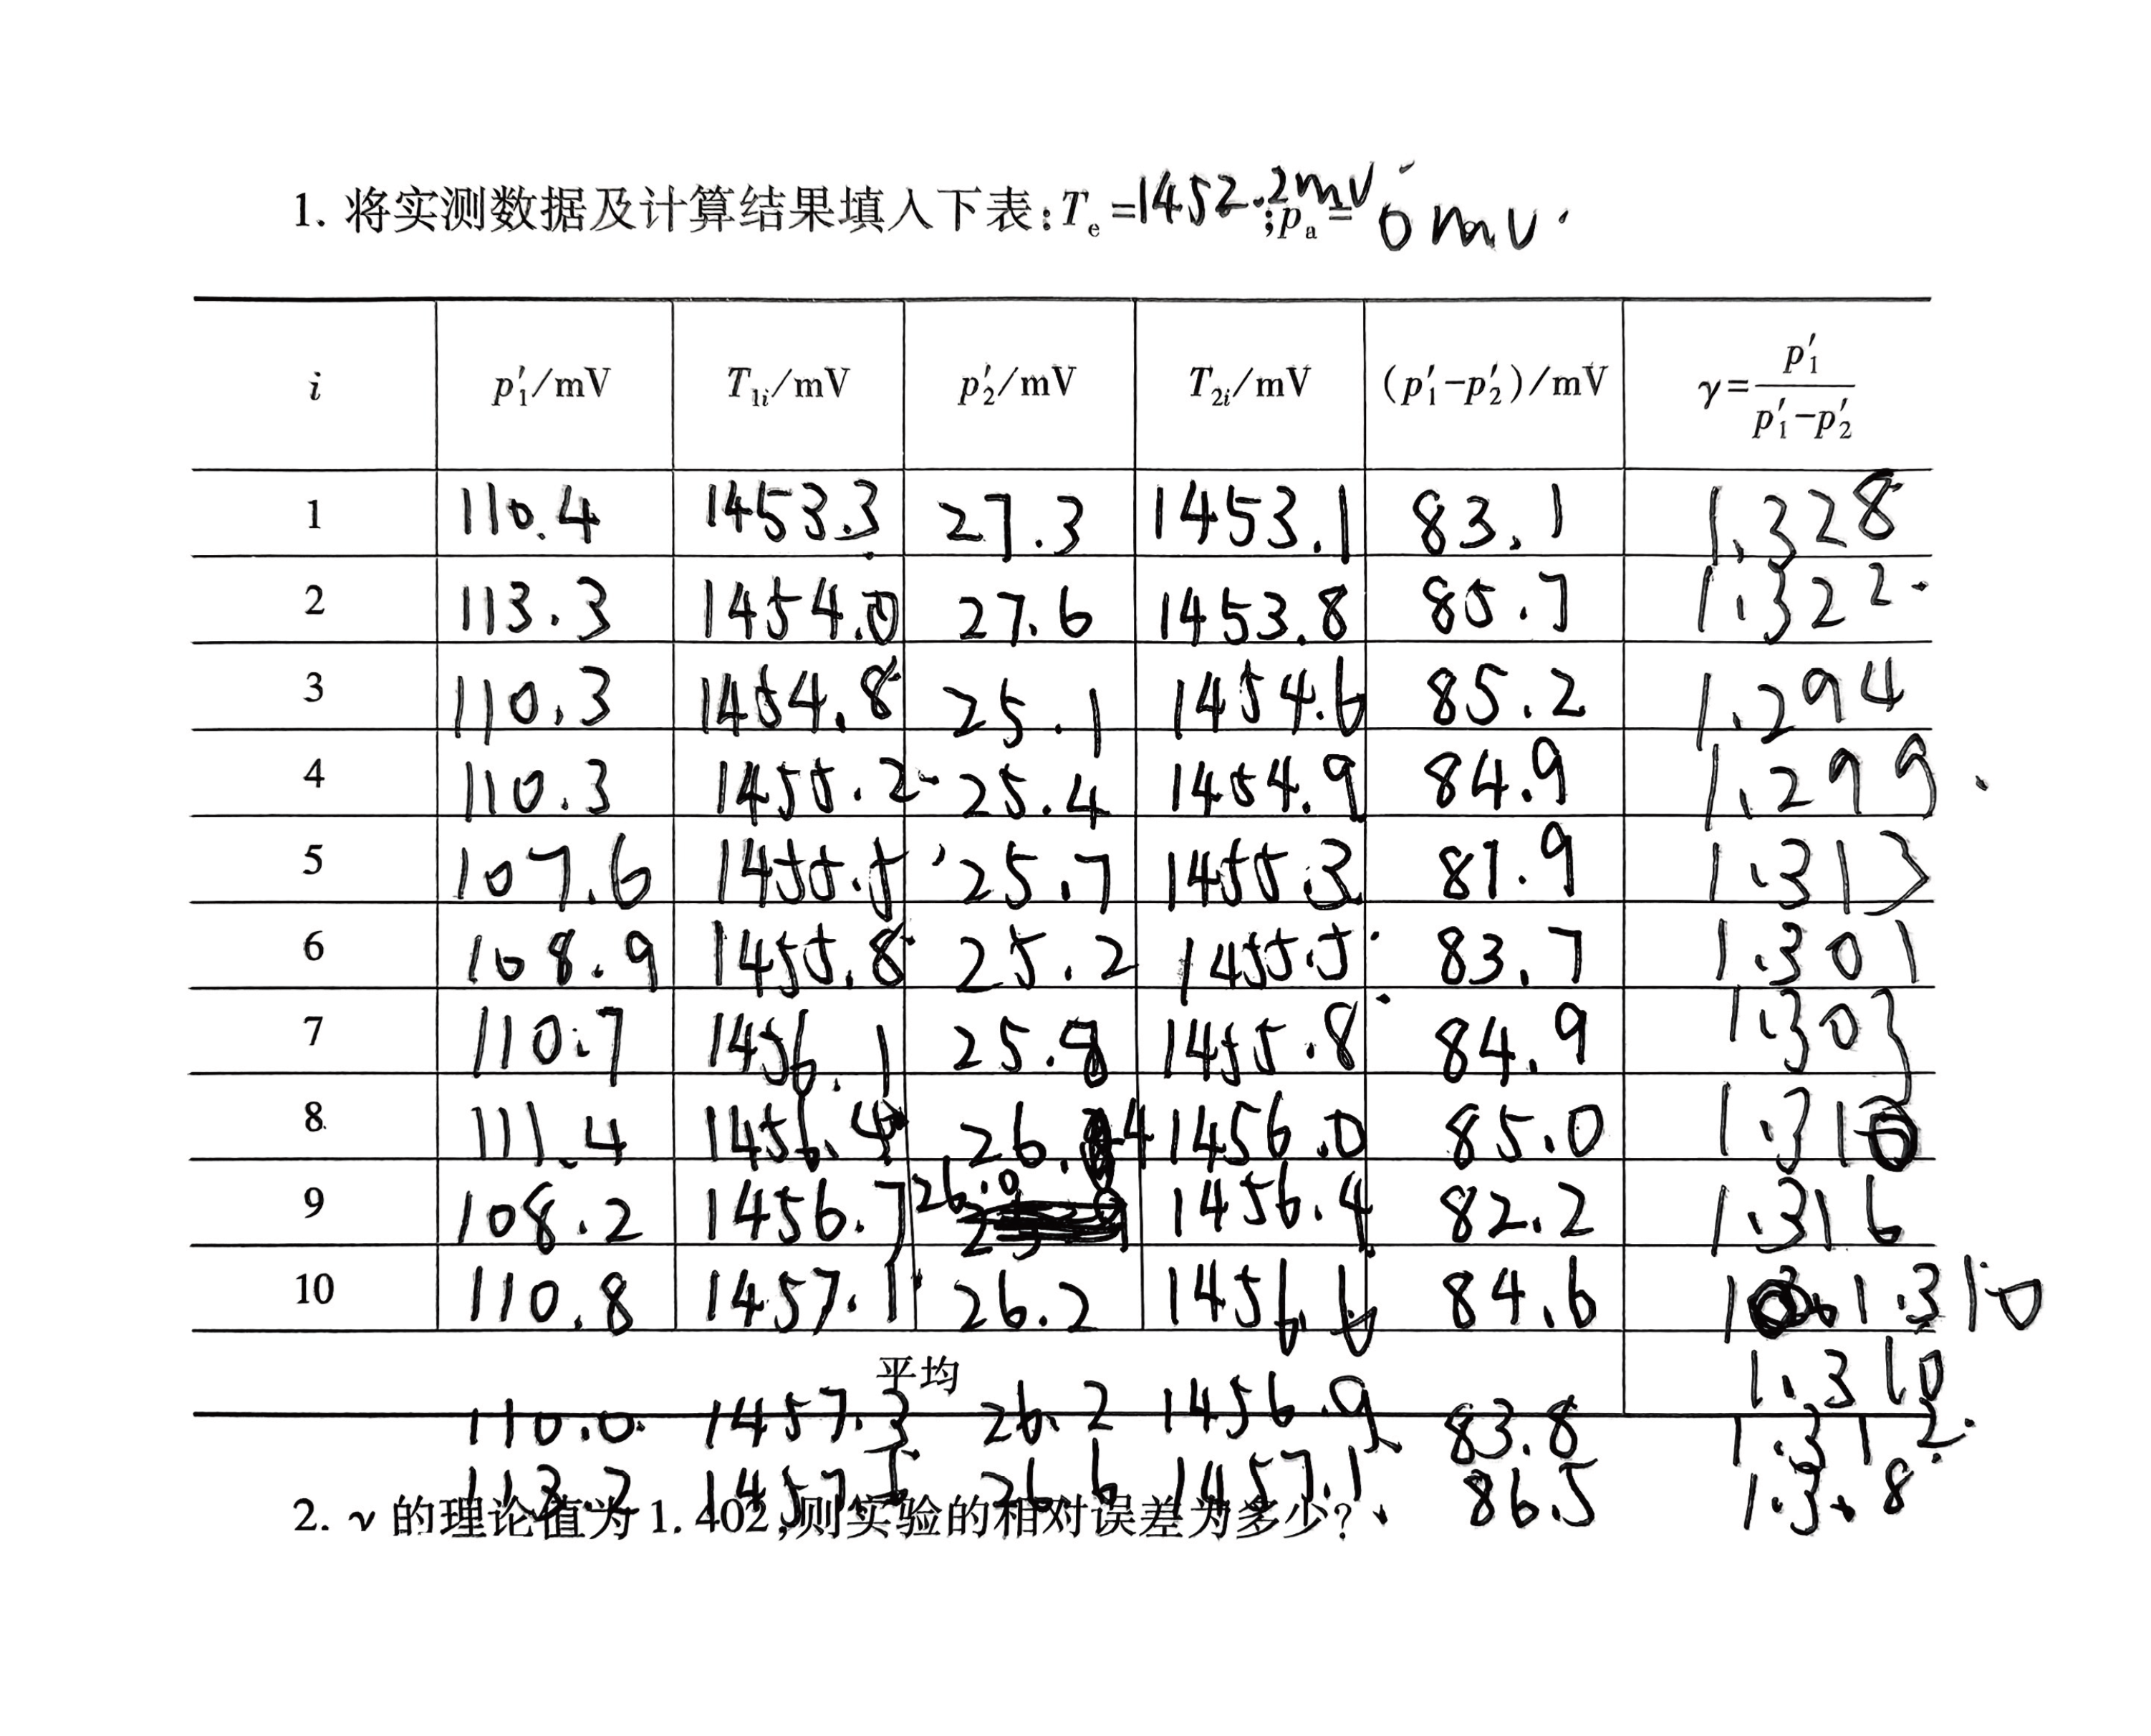
\includegraphics[width=0.7\linewidth]{数据表格}
		\caption{数据表格}
	\end{figure} 重复十次实验,对每组实验求得的$\gamma$取平均值。求得$\overline{\gamma}=1.31$,计算与理论值$1.402$的相对误差
	\[E_{x} = \frac{1.402-1.310}{1.402}=6.5\%\]

	\subsection*{[注意事项]}
	\par 1.旋转活塞时应慢,防止活塞被折断。
	\par 2.压入气体时若太多,则仪器不密封造成的误差会增大,若太少,则实验效果不明显,以使电压表示数为$120mV$最佳。
	\par 3.打开放气活塞待声音消失后应当立刻关上活塞,否则实验结果偏小。
	\subsection*{[考察题与思考题]}
	\subsubsection*{考察题第四题}
	\par 由于打入的气体不均匀,仪器测量的下半部分压强比较大,若读取的时间间隔太小,$p_1^{\prime}$的值会偏大;由于释放完气体需要等待一段时间气体吸热压强增大,故读取时间过快的话,$p_2^{\prime}$会偏小。
	\par 如果时间间隔很长,由于不可能做到百分之一百密封,故$p_1^{\prime}和p_2^{\prime}$都会偏小,对实验有影响但影响未知。
	\subsubsection*{思考题第三题}
	\par 是室内空气。应该没有影响。
\end{document}